\title{The Standard Vectors} 
\subtitle{\SubTitleName}
\institute[]{\Course}
\author{\Instructor}
\maketitle

\frame{\frametitle{Topics and Learning Objectives}

\Emph{Topics} \\

\TopicStatement

\begin{itemize}
    \item the \Emph{standard vectors} and the \Emph{standard matrix}
    % \item Two and three dimensional transformations in more detail.  
    % \item \Emph{Onto} and \Emph{one-to-one} transformations. 
\end{itemize}

\vspace{0.5cm}
    
    \LO\\
    
    \LearningObjectiveStatement
    
    \begin{itemize}
        \item construct the matrix of a linear transformations using standard vectors
        % \item Characterize linear transformations as onto and/or one-to-one. 
        % \item Solve linear systems represented as linear transforms.
        % \item Express linear transforms in other forms, such as as matrix equations or as vector equations.
    \end{itemize}



\vspace{0.25cm} 

%\Emph{Motivating Question} \\

%A linear transformation  $ T \;:\;  \mathbb R ^2 \mapsto \mathbb R ^{3} $  satisfies 
%\begin{equation*}
%T \begin{pmatrix} 1 \\ 0 \end{pmatrix} = \begin{pmatrix} 5 \\ -7 \\ 2  \end{pmatrix},
%\qquad 
%T \begin{pmatrix*}[r]  0 \\ 1 \end{pmatrix*} = \begin{pmatrix*}[r] -3 \\ 8 \\ 0  
%\end{pmatrix*}
%\end{equation*}
%Is there a matrix that represents $ T_A$? If so, what could it be equal to? 
}






\frame{\frametitle{Definition: The Standard Vectors}

    A \Emph{standard vector}, $\vec e_i$ is a vector in $\mathbb R^n$, in which every entry of the vector is zero, except for entry $i$, which is equal to 1. 
    
    \vspace{.25cm} 
    
    For example, in $\mathbb R^3$, 
    
        $$\onslide<2->{\vec e_1 = \begin{pmatrix} 1\\0\\0\end{pmatrix}} \qquad 
        \onslide<3->{\vec e_2 = \begin{pmatrix} 0\\1\\0\end{pmatrix}} 
        \qquad 
        \onslide<4->{\vec e_3 = \begin{pmatrix} 0\\0\\1\end{pmatrix}} $$

} 


\frame{\frametitle{A Property of the Standard Vectors}

    \Emph{Note}: if $A$ is an $m\times n$ matrix with columns $\vec v_1,\vec v_2,\ldots, \vec v_n$, then
    $$A\vec e_i = \vec v_i, \text{ for } i=1,2,\ldots,n$$
    \onslide<2->{So multiplying a matrix by $\vec e_i$ gives column $i$ of $A$.}\\[6pt]

    \onslide<3->{\Emph{Example}}\\
    $$\onslide<4->{\spalignmat{1 2 3; 4 5 6; 7 8 9} \vec e_2 
    = }
    \onslide<5->{\spalignmat{1 2 3; 4 5 6; 7 8 9} \begin{pmatrix} 0\\1\\0 \end{pmatrix} =}
    \onslide<6->{0\begin{pmatrix} 1\\4\\7\end{pmatrix} + 1 \begin{pmatrix} 2\\5\\8 \end{pmatrix} + 0 \begin{pmatrix} 3\\6\\9 \end{pmatrix} = }
    \onslide<7->{ \begin{pmatrix} 2\\5\\8 \end{pmatrix} }
    $$
    \begin{itemize}
        \item \onslide<8->{Multiplying the matrix by $\vec e_2$ gave us the second column of the matrix.}
        \item \onslide<9->{We can use this concept to construct the standard matrix of a transform.}
    \end{itemize}

    
}




\frame{\frametitle{The Standard Matrix}

\begin{center}\begin{tikzpicture} \node [mybox](box){\begin{minipage}{0.75\textwidth}
    \vspace{4pt}

    Let $  T $ be a linear transformation that maps $ \mathbb R ^n$ to $\mathbb R ^m$. Then there is a unique matrix $ A$ such that 
    \onslide<2->{
    \begin{equation*}
        T ( \vec x ) = A \vec x, \qquad \vec x\in \mathbb R ^{n}. 
    \end{equation*}
    } \onslide<3->{
    \hspace{-.4cm}Also, $ A$ is a $ m \times n$, and column $j$ is the vector $ T (\vec e _j)$.} \onslide<4->{In other words, $A = \begin{pmatrix} T (\vec e_1) & T(\vec e_2)  & \cdots  & T (\vec e_n) \end{pmatrix}$.} 
    
    \end{minipage}}; \node[fancytitle, right=10pt] at (box.north west) {Theorem}; \end{tikzpicture}\end{center}

    \begin{itemize}
        \item<4-> Most introductory linear algebra textbooks prove the uniqueness component of this theorem.
        \item<5-> The matrix $ A$ is the \Emph{standard matrix} for a linear transformation.  
    \end{itemize}

}



\frame{\frametitle{Standard Matrix for a Counterclockwise Rotation}

    What is the standard matrix of the transform $T : \R^2 \rightarrow \R^2$ defined by:
    \begin{center}
        $T(\vec x) = \vec x \text{ \textit{rotated counterclockwise by angle} } \theta$?
    \end{center}
    \onslide<2->{Our standard matrix, $A$. will have two columns and two rows.}
    \onslide<3->{To construct $A$ we can use the theorem from the previous slide: $$
        A = \begin{pmatrix}
        T (\vec e_1) & T(\vec e_2) 
    \end{pmatrix}$$ We need to determine $T (\vec e_1)$ and $T (\vec e_2)$. }

}

\frame{\frametitle{Calculating $T(\vec e_1)$}

    Our goal now is to determine what happens to $\vec e_1$ after it is rotated counterclockwise by $\theta$ radians. 
    
    \begin{tikzpicture}[scale=3]
    \coordinate (O) at (0,0);  % variable for origin
    % axes
    \onslide<2->{
    \draw[-, thin,black] (-0.5,0) -- (1.5,0) node[anchor=north] {$x_1$};
    \draw[-, thin,black] (0,-0.3) -- (0.0,1.15) node[anchor=east] {$x_2$};
    }
    % vectors    
    \onslide<3->{
    \draw[->,Black,ultra thick,-stealth,rotate=0] (O) -- (1,0) node[anchor=south west ] {$\vec e_1$};
    }
    \onslide<4->{
    \draw[->,DarkBlue,ultra thick,-stealth,rotate=0] (O) -- (.707,0.707); \draw[DarkBlue] (.6,.6) node[anchor=south west] {$T(\vec e_1) = \begin{pmatrix} x\\y \end{pmatrix}$};     
    \draw[DarkBlue] (0.35,0.18) node[anchor= west] {$\theta$};
    \draw[ultra thick, DarkBlue, ->] (0.35,0) arc (0:45:0.35);
    \draw[thin, DarkBlue, dashed] (1,0) arc (0:90:1);
    }

    \onslide<5->{
    % horiz comp drop line
    \draw[dashed, thin,DarkBlue] (0.707,0.707) -- (0.707,0);
    \draw[-, thin,DarkBlue] (0.707,0.1) -- (0.6,0.1);
    \draw[-, thin,DarkBlue] (0.6,0) -- (0.6,0.1);
    % vert comp drop line
    \draw[dashed, thin,DarkBlue] (0.707,0.707) -- (0,0.707);
    \draw[-, thin,DarkBlue] (0.1,0.707) -- (0.1,0.6);
    \draw[-, thin,DarkBlue] (0,0.6) -- (0.1,0.6); 
    }
    
    % hoiz and vert components
    \onslide<6->{
    \draw [decorate, ultra thick, DarkRed, decoration = {calligraphic brace}]  (0.707,-0.05) -- (0,-0.05);    
    \draw[black] (0.35,-0.1) node[anchor= north] {$x$};
    \draw [decorate, ultra thick, DarkRed, decoration = {calligraphic brace}]  (-0.05,0) -- (-0.05,0.707);    
    \draw[black] (-0.15,0.45) node[anchor= north] {$y$};    
    }
    
    % Derivation on right 
    \onslide<7->{
    \draw[black] (2.4,1.1) node[anchor= north] {$\cos\theta = \frac{x}{r}, \quad \sin\theta = \frac{y}{r}$};}
    \onslide<8->{
    \draw[black] (2.12,0.8) node[anchor= north] {But $r = 1$, so};
    \draw[black] (2.4,0.5) node[anchor= north] {$x = \cos\theta, \quad y = \sin \theta $};
    }
    \onslide<9->{
    \draw[black] (2.6,0.25) node[anchor= north] {$ \Rightarrow T(\vec e_1) = \begin{pmatrix} x \\  y \end{pmatrix} =
    \begin{pmatrix} \cos\theta \\  \sin \theta\end{pmatrix} $};
    }
\end{tikzpicture}

    \onslide<10->{So if $
        A = \begin{pmatrix}
        T (\vec e_1) & T(\vec e_2) 
    \end{pmatrix}$, then the \Emph{first} column of $A$ is $\begin{pmatrix} \cos \theta \\ \sin \theta \end{pmatrix}$.
    }
}




\frame{\frametitle{Calculating $T(\vec e_2)$}

    We can use a similar process to determine what happens to $\vec e_2$ after it is rotated counterclockwise by $\theta$ radians. 
    
    \begin{tikzpicture}[scale=3]
    \coordinate (O) at (0,0);  % variable for origin
    % axes
    \onslide<2->{
    \draw[-, thin,black] (-1.5,0) -- (0.45,0) node[anchor=north] {$x_1$};
    \draw[-, thin,black] (0,-0.3) -- (0.0,1.25) node[anchor=east] {$x_2$};
    }
    % vectors    
    \onslide<3->{
    \draw[->,Black,ultra thick,-stealth,rotate=0] (O) -- (0,1) node[anchor=south west ] {$\vec e_2$};
    }
    \onslide<4->{
    \draw[->,DarkBlue,ultra thick,-stealth,rotate=0] (O) -- (-.707,0.707); \draw[DarkBlue] (-1.7,.6) node[anchor=south west] {$T(\vec e_2) = \begin{pmatrix} x\\y \end{pmatrix}$};     
    \draw[DarkBlue] (-0.25,0.42) node[anchor= west] {$\theta$};
    \draw[ultra thick, DarkBlue, ->] (0,0.35) arc (90:135:0.35);
    \draw[thin, DarkBlue, dashed] (0,1) arc (90:180:1);
    }

    \onslide<5->{
    % horiz comp drop line
    \draw[dashed, thin,DarkBlue] (-0.707,0.707) -- (-0.707,0);
    \draw[-, thin,DarkBlue] (-0.707,0.1) -- (-0.6,0.1);
    \draw[-, thin,DarkBlue] (-0.6,0) -- (-0.6,0.1);
    % vert comp drop line
    \draw[dashed, thin,DarkBlue] (-0.707,0.707) -- (0,0.707);
    \draw[-, thin,DarkBlue] (-0.1,0.707) -- (-0.1,0.6);
    \draw[-, thin,DarkBlue] (0,0.6) -- (-0.1,0.6); 
    }
    
    % hoiz and vert components
    \onslide<6->{
    \draw [decorate, ultra thick, DarkRed, decoration = {calligraphic brace}]  (0,-0.05) -- (-0.707,-0.05);    
    \draw[black] (-0.35,-0.1) node[anchor= north] {$x$};
    \draw [decorate, ultra thick, DarkRed, decoration = {calligraphic brace}]  (0.05,0.707) -- (0.05,0);    
    \draw[black] (0.18,0.45) node[anchor= north] {$y$};    
    }
    
    % Derivation on right 
    \onslide<7->{
    \draw[black] (1.35,1.4) node[anchor= north] {$\sin\theta = -\frac{x}{r}, \quad \cos\theta = \frac{y}{r}$};
    \draw[black] (1.65,1.1) node[anchor= north] {Note that $x < 0$ for $0< \theta < \pi/2$.};
    }
    \onslide<8->{
    \draw[black] (1.05,0.8) node[anchor= north] {And $r = 1$, so};
    \draw[black] (1.4,0.5) node[anchor= north] {$x = -\sin\theta, \quad y = \cos \theta $};
    }
    \onslide<9->{
    \draw[black] (1.6,0.25) node[anchor= north] {$ \Rightarrow T(\vec e_2) = \begin{pmatrix} x \\  y \end{pmatrix} =
    \begin{pmatrix} -\sin\theta \\  \cos \theta\end{pmatrix} $};
    }
\end{tikzpicture}

    \onslide<10->{So if $
        A = \begin{pmatrix}
        T (\vec e_1) & T(\vec e_2) 
    \end{pmatrix}$, then the \Emph{second} column of $A$ is $\begin{pmatrix} - \sin \theta \\ \cos \theta \end{pmatrix}$.
    }
}





\frame{\frametitle{The Standard Matrix for Counterclockwise Rotations}

    \onslide<2->{The standard matrix for a counterclockwise rotation about the origin in $\mathbb R^2$ has the form}
    \onslide<3->{
    $$
        A = \begin{pmatrix}
        T (\vec e_1) & T(\vec e_2) 
    \end{pmatrix}$$ 
    }
    \onslide<4->{But we found that 
        $$T(\vec e_1) = \begin{pmatrix}  \cos \theta \\ \sin \theta \end{pmatrix}, \quad T(\vec e_2) = \begin{pmatrix} - \sin \theta \\ \cos \theta \end{pmatrix}$$
    }
    \onslide<5->{Therefore, the standard matrix is 
    $$A = \begin{pmatrix}  \cos \theta & - \sin \theta \\ \sin \theta & \cos \theta \end{pmatrix}$$}

}

\frame{\frametitle{Verifying our Results}

    \onslide<2->{Is our matrix for a counterclockwise rotation about the origin in $\mathbb R^2$ correct?}
    \onslide<3->{If it is, then we would expect that, for example, when $\theta = \pi/2$ radians that, 
    $$v = \begin{pmatrix} 2\\0\end{pmatrix} \to \begin{pmatrix} 0\\2\end{pmatrix}$$ Does it?
    }
    \onslide<4->{When $\theta = \pi/2$, we have }
    $$\onslide<5->{A = \begin{pmatrix}  \cos \pi/2 & - \sin \pi/2 \\ \sin \pi/2 & \cos \pi/2 \end{pmatrix} = } \onslide<6->{\begin{pmatrix} 0&-1\\1&0\end{pmatrix}}$$
    \onslide<7->{Therefore }
    \onslide<8->{$$T(v) = Av = \begin{pmatrix} 0&-1\\1&0\end{pmatrix} \begin{pmatrix} 2\\0 \end{pmatrix} = \begin{pmatrix} 0\\2\end{pmatrix}$$}
    \onslide<9->{The result in this case is what we needed, so it seems our matrix is correct.}
}


\frame{\frametitle{Standard Matrix for a Clockwise Rotation}

    \onslide<2->{A similar process for clockwise rotations reveals that
    \begin{center}
        $T(\vec x) = \vec x \text{ \textit{rotated clockwise by angle} } \theta = A \vec x$
    \end{center}
    }
    \onslide<3->{where
    $$A = \begin{pmatrix} T (\vec e_1) & T(\vec e_2) \end{pmatrix} = \begin{pmatrix} \cos\theta & \sin\theta \\ -\sin\theta & \cos\theta \end{pmatrix}$$ 
    }
    \onslide<4->{
    \Emph{Example}
    \begin{center}
    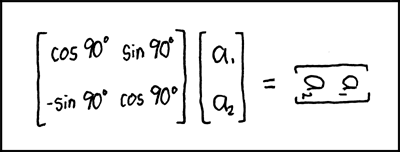
\includegraphics[width=0.5\textwidth]{Chapter1/images/XKCDmatrix_transform.png} \\{\small \textit{https://xkcd.com/184}}
    \end{center}
    }
    \vfill 
}








% \frame{\frametitle{Example: Constructing a Standard Matrix}

%     Define a linear transformation by $$ T (x_1 ,x_2) = (3x_1 + x_2 , 5x_1 + 7 x_2 , x_1 + 3 x_2 )$$ Is $T$ one-to-one?  Is $T$ onto?  



% }

\frame{\frametitle{Summary}

    \SummaryLine \vspace{4pt}
    \begin{itemize}\setlength{\itemsep}{8pt}
            \item standard vectors $\vec e_i$
            \item construct the standard matrix of a linear transform in $\mathbb R^n$ using the result that $A = \begin{pmatrix}
        T (\vec e_1) & T(\vec e_2)  & \cdots  & T (\vec e_n)
    \end{pmatrix}$
            \item constructing the standard matrix for a rotation matrix
    \end{itemize}
    \vspace{12pt}
    Note that
    \begin{itemize}
        \item The rotation matrix was just one of many standard matrices that are introduced in introductory linear algebra textbooks.
        \item There are other standard matrices for transformations that we will explore.
    \end{itemize}
}


